\documentclass[main.tex]{subfiles}


\begin{document}

\begingroup

\renewcommand{\cleardoublepage}{}

\renewcommand{\clearpage}{}
\newpage
\chapter{Perception Function Documentation}

\section{Introduction}
\chapterauthor{Jan-Frederik Stock}
The task of the perception group was to use the available image data to gather as much information as possible about the perceived scene. In the following chapter, the tools and software used and created by the perception group will be described. These include descriptions of the pipelines and annotators used in \textit{RoboSherlock}, the image processing framework used by the perception group, as well as tools for classification.

\section{RoboSherlock}
		\chapterauthor{Jan-Frederik Stock}
The main framework the perception group is working with is \textit{RoboSherlock} \footnote{\url{http://www.robosherlock.org/}}. RoboSherlock is a software, that uses multiple expert systems called annotators on input image data. Each annotator performs a specific task, for example searching for objects in a given picture. All annotators write their results to a public data structure.\\
		
\textit{RoboSherlock} works by executing all of these annotators in a predefined order. This order is called a pipeline. There can be pipelines for different purposes, in the perception groups case for detecting objects and detecting surfaces. Each pipeline can have different annotators. Thus, \textit{RoboSherlock} can be customized to achieve many different image processing tasks.

		\section{rs\_perception}\label{rs_perception}
		\chapterauthor{Leonidas Paniago}
To understand this chapter, the term pipeline needs to be further defined.The term pipeline is often used in computer science for the successive execution of processes
In \textit{RoboSherlock}, the pipeline fulfills a similar task. The processing of camera output is divided into several tasks that have to be executed one after the other.
Each task in the pipeline is called Annotator and it has an own purpose, here is a list of some tasks: 
		\begin{itemize}
			\item Annotation
			\item Detection
			\item Filter
			\item Flow control
			\item Query answering
			\item Recognition 
			\item Segmentation
			\item Tracking
		\end{itemize}		
The pipeline order is determined by the already processed information and the needed information for the next step.
Each annotator contains changeable parameter that enables customization to the given tasks. All main pipelines are included in \href{https://github.com/SUTURO/suturo_perception/tree/master/rs_perception}{rs\_perception}

			\subsection{Pipeline: hsrb\_1ms}

The main pipeline for detecting and identifying objects with \textit{RoboSherlock} consists of the following annotators in order:  
\begin{itemize}
	\item CollectionReader : Takes care of the Camera  Input

	\begin{minipage}[t]{\textwidth}
	\item ImagePreprocessor : Prepares image for further processing and implement image filters
		\begin{figure}[H]
   			 \centering
    			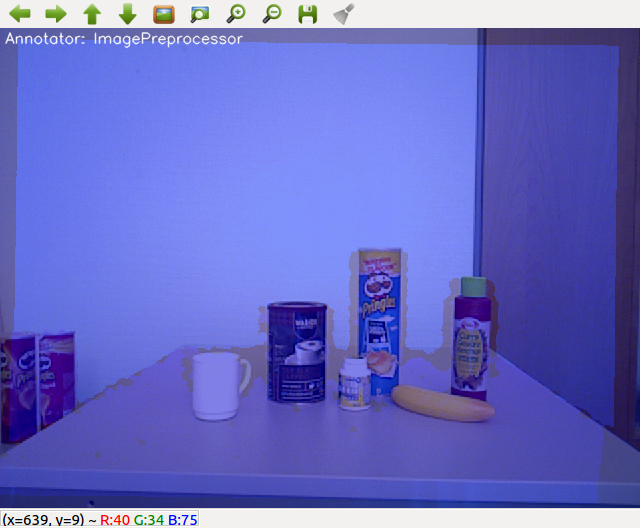
\includegraphics[width=0.5\textwidth]{pictures/2d/ImagePreProcessor.png}
   			 \caption{ImagePreprocessor}
  		\end{figure}
	\end{minipage}

	\begin{minipage}[t]{\textwidth}
	\item SuturoRegionFilter : Remove all points that are not in the defined Regions 
		\begin{figure}[H]
   			 \centering
    			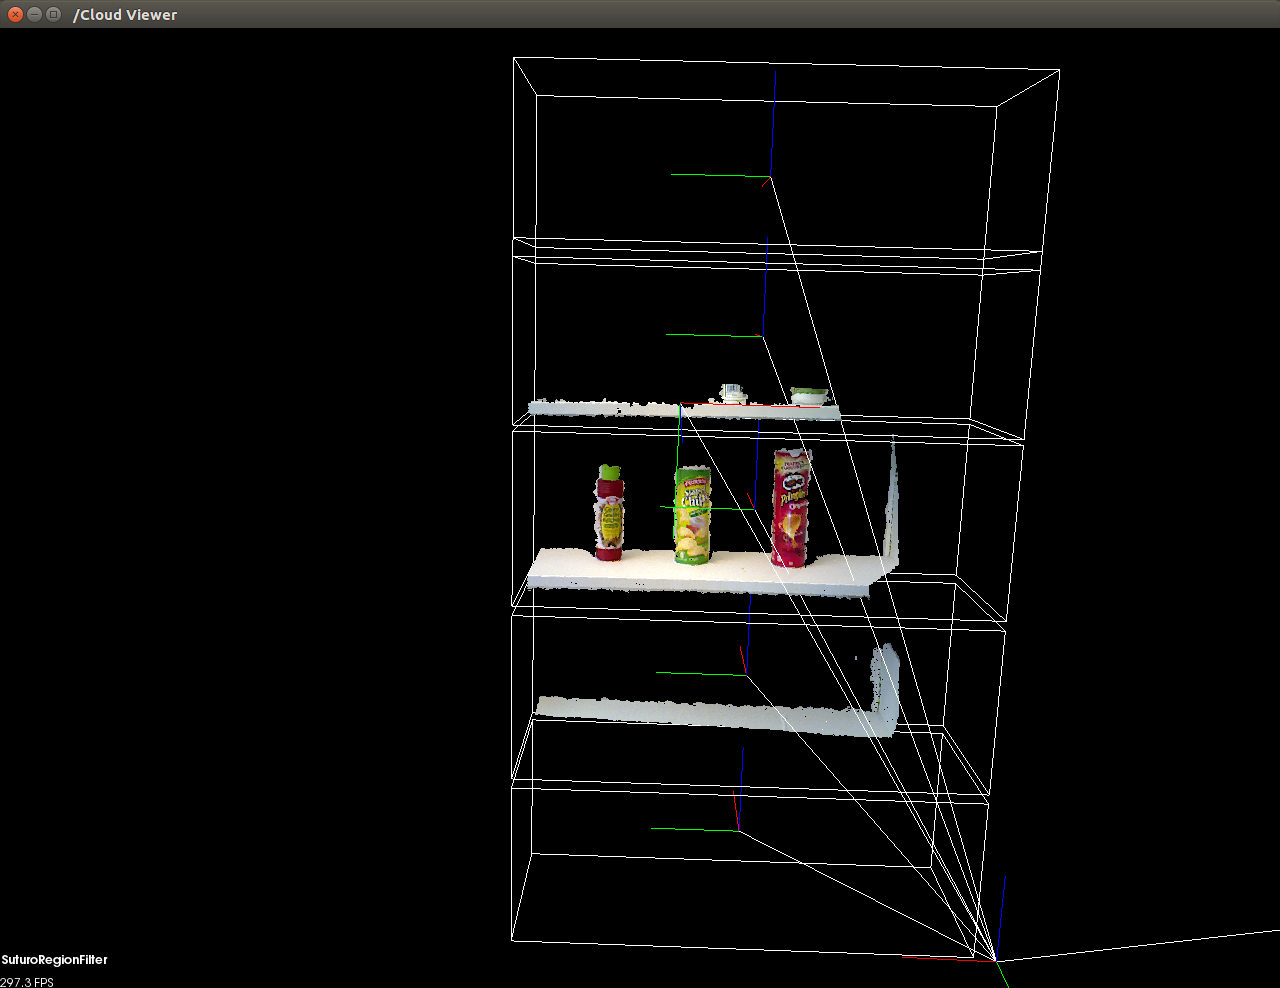
\includegraphics[width=0.5\textwidth]{pictures/pcl/RegionFilter.png}
   			 \caption{SuturoRegionFilter}
  		\end{figure}
	\end{minipage}

	\begin{minipage}[t]{\textwidth}
	\item NormalEstimator : Estimate Surface Normals in a PointCloud 
		\begin{figure}[H]
   			 \centering
    			 \subfigure[NormalEstimator]{%
           		 \includegraphics[width=0.5\textwidth]{pictures/2d/NormalEstimator.png}
			 }%
       			 \subfigure[NormalEstimator]{%
           		 \includegraphics[width=0.5\textwidth]{pictures/pcl/NormalEstimator.png}
       			 }
   			 \caption{NormalEstimator}
  		\end{figure}
	\end{minipage}

	\begin{minipage}[t]{\textwidth}
	\item PlaneAnnotator : Search for Horizontal Planes in which the search location for Objects is set
		\begin{figure}[H]
   			 \centering
    			 \subfigure[PlaneAnnotator]{%
           		 \includegraphics[width=0.5\textwidth]{pictures/2d/PlaneAnnotator.png}
        			 }%
       			 \subfigure[PlaneAnnotator]{%
           		 \includegraphics[width=0.5\textwidth]{pictures/pcl/PlaneAnnotator.png}
        			 }
   			 \caption{PlaneAnnotator}
  		\end{figure}
	\end{minipage}
	
	\begin{minipage}[t]{\textwidth}
	\item PointCloudClusterExtractor : Extract all Points found in the PointCloud that are perpendicular to the Plane 
		\begin{figure}[H]
   			 \centering
    			 \subfigure[PointCloudClusterExtractor]{%
            		\includegraphics[width=0.5\textwidth]{pictures/2d/PointCloudClusterExtractor.png}
        			}%
        			\subfigure[PointCloudClusterExtractor]{%
           		 \includegraphics[width=0.5\textwidth]{pictures/pcl/PointCloudClusterExtractor.png}
        			}
   			 \caption{PointCloudClusterExtractor}
  		\end{figure}
	\end{minipage}

	\begin{minipage}[t]{\textwidth}
	\item ClusterColorHistogramCalculator : Calculate the individual color quantity in relation to all colors on the cluster   
		\begin{figure}[H]
   			 \centering
    			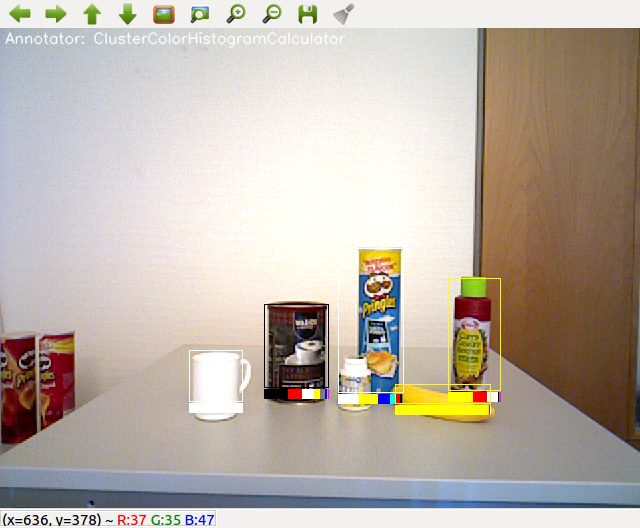
\includegraphics[width=0.5\textwidth]{pictures/2d/ClusterColorHistogramAnnotator.png}
   			 \caption{ClusterColorHistogramCalculator}
  		\end{figure}
	\end{minipage}

	\begin{minipage}[t]{\textwidth}
	\item Cluster3DGeometryAnnotator : Extracts basic attributes of cluster like initial pose, semantic size and 3D bounding box 
		\begin{figure}[H]
   			 \centering
    			 \subfigure[Cluster3DGeometryAnnotator]{%
            		\includegraphics[width=0.5\textwidth]{pictures/2d/Cluster3DGeometryAnnotator.png}
        			}%
        			\subfigure[Cluster3DGeometryAnnotator]{%
           		 \includegraphics[width=0.5\textwidth]{pictures/pcl/Cluster3DGeometryAnnotator.png}
        			}
    			 
   			 \caption{Cluster3DGeometryAnnotator}
  		\end{figure}
	\end{minipage}

	\begin{minipage}[t]{\textwidth}
	\item SuturoShapeAnnotator : Detects the shape of the object (cylinder, sphere, box)
		\begin{figure}[H]
   			 \centering
    			 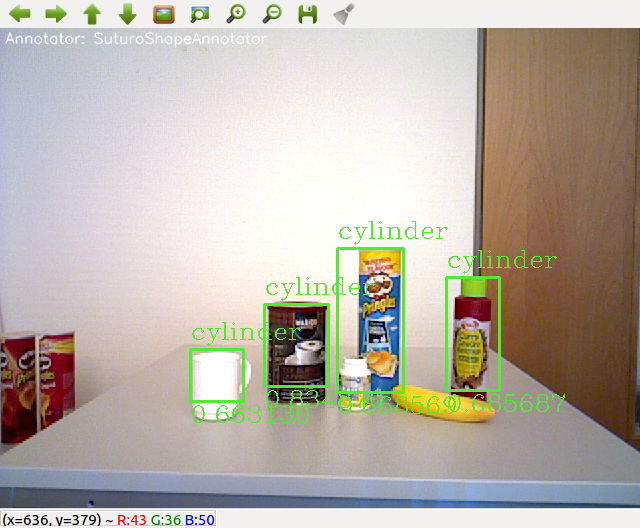
\includegraphics[width=0.5\textwidth]{pictures/2d/SuturoShapeAnnotator.png}
   			 \caption{SuturoShapeAnnotator}
  		\end{figure}
	\end{minipage}

	\item RegionAnnotator : Further restriction on which areas will be used based on defined Regions 
	\item CaffeAnnotator : Deep learning method for Object recognition based on prerecorded Images 

	\begin{minipage}[t]{\textwidth}
	\item KnnAnnotator : Uses K-Nearest-Neighbor for classification of Objects 
		\begin{figure}[H]
   			 \centering
    			 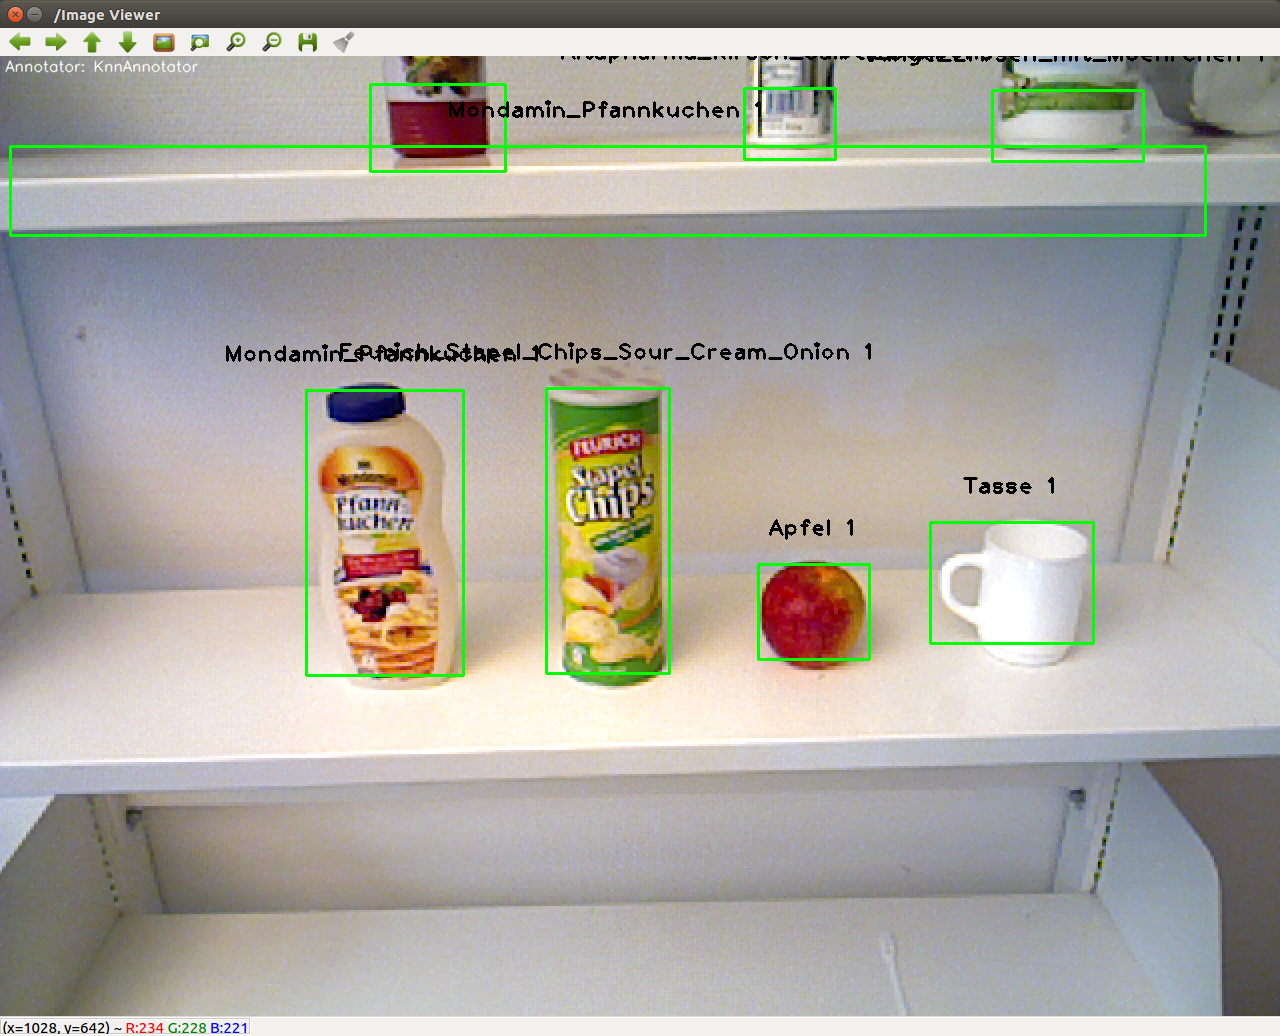
\includegraphics[width=0.5\textwidth]{pictures/2d/KnnAnnotator.png}
   			 \caption{KnnAnnotator}
  		\end{figure}
	\end{minipage}
\end{itemize}



			\subsection{Pipeline: hsrb\_planes} 
This pipeline is used to detect a shelf door. It is used to find a plane that is parallel to the z-axis of the camera.
\begin{itemize}
	\item CollectionReader : Takes care of the camera input
	\item ImagePreprocessor : Prepares image for further processing and implement image filters  
	\item PointCloudFilter : Filters points that are not in the range of the given parameters for X, Y and Z axes out of the cloud
	\item NormalEstimator : Estimate surface normal's in a PointCloud 
	\item PlaneAnnotator : Finds a plane in the current scene and saves it into the CAS.
	\item PointCloudClusterExtractor : Extracts all points found in the PointCloud that are perpendicular to the plane 
\end{itemize}

			\subsection{Pipeline: storage\_suturo} 
Pipeline for storing camera images in MongoDB, all saved scenes can be replayed for testing without the HSR and have the same functionality. 
\begin{itemize}
	\item CollectionReader : Takes care of the camera input
	\item ImagePreprocessor : Prepares image for further processing and implement image filters 
	\item StorageWriterSuturo :  Records defined camera topics into the MongoDB
\end{itemize}

		\section{actionserver}
		\chapterauthor{Leonidas Paniago}
The \href{https://github.com/SUTURO/suturo_perception/tree/master/actionserver}{action server} contains the server responsible for the pipeline execution they are based on the \href{http://wiki.ros.org/actionlib}{ROS Client-Server Interaction} and it works by providing three callable actions types:
\begin{itemize}
	\item Goal : A specific defined task 
	\item Feedback : Information about the goal execution  
	\item Result : The goal final result 
\end{itemize}
This approach facilitates the communication with perception by offering a clear interface.
Each server provides the same actions with different results based on their functionality.
The implemented clients are not needed for the HSR execution than knowledge has its own implementation, they are mainly used for testing and troubleshooting. 
Both servers give the same message output \href{https://github.com/SUTURO/suturo_resources/blob/master/messages/suturo_perception_msgs/msg/ObjectDetectionData.msg}{ObjectDetectionData.msg} consisting of : 

	\begin{itemize}
	\item Class
	\item Shape (Cylinder, Sphere, Box)
	\item Colour
	\item Position
	\item Height
	\item Depth
	\item Width
	\item Orientation
	\end{itemize}

			\subsection{ExtractObjectInfoClient}
Call \texttt{ExtractObjectInfoServer} and wait until the result arrives or the time out runs out. \texttt{region} can be set to limit the perception of objects to a specific region, if \texttt{default} is set the region filter will be disabled. The client can be started by calling : \texttt{rosrun actionserver ExtractObjectInfoClient}

			\subsection{ExtractObjectInfoServer}
Receives a goal from Client and passes on to \texttt{SuturoProcessManager}, checks for results, and publishes them under \texttt{perception\_actionserver/result}. 
			\begin{figure}[H]
   			 \centering
    			 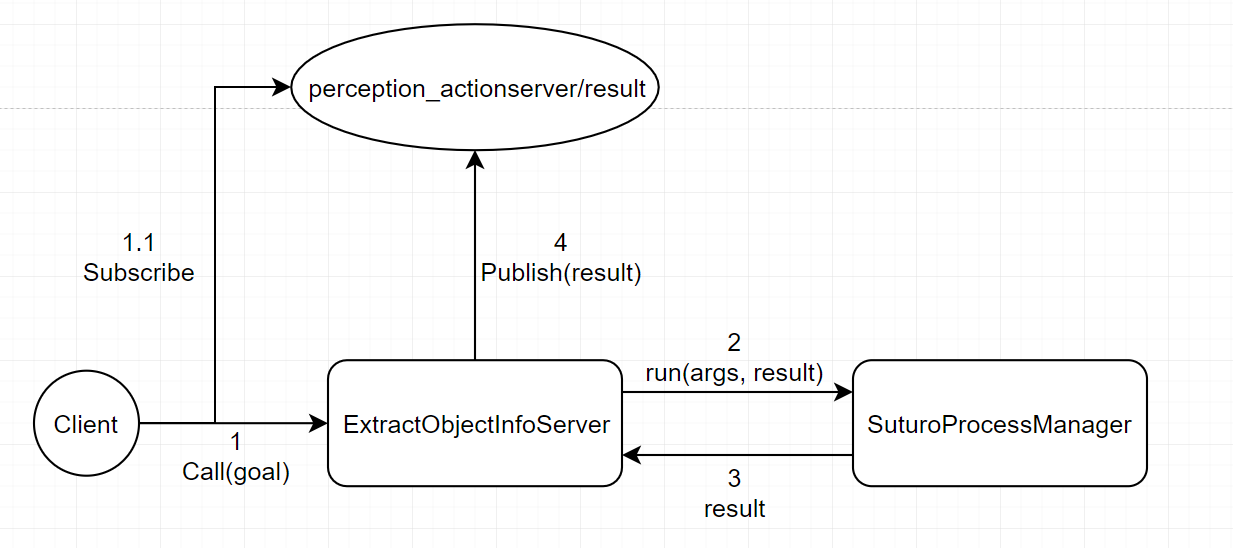
\includegraphics[width=1\textwidth]{pictures/perception/suturo_ExtractObjectInfoServer.png}
   			 \caption{ExtractObjectInfoServer}
  			\end{figure}

			\subsection{ExtractPlaneInfoClient}
Call ExtractPlaneInfoServer and wait until the result arrives or the time out runs out. This client has no additional parameters.
The client can be started by calling : \texttt{rosrun actionserver ExtractPlaneInfoClient}.

			\subsection{ExtractPlaneInfoServer}
Receives a goal from Client and pass on to SuturoProcessManager, checks for result and publishes it under \texttt{perception\_actionserver\_plane/result}.
			\begin{figure}[H]
   			 \centering
    			 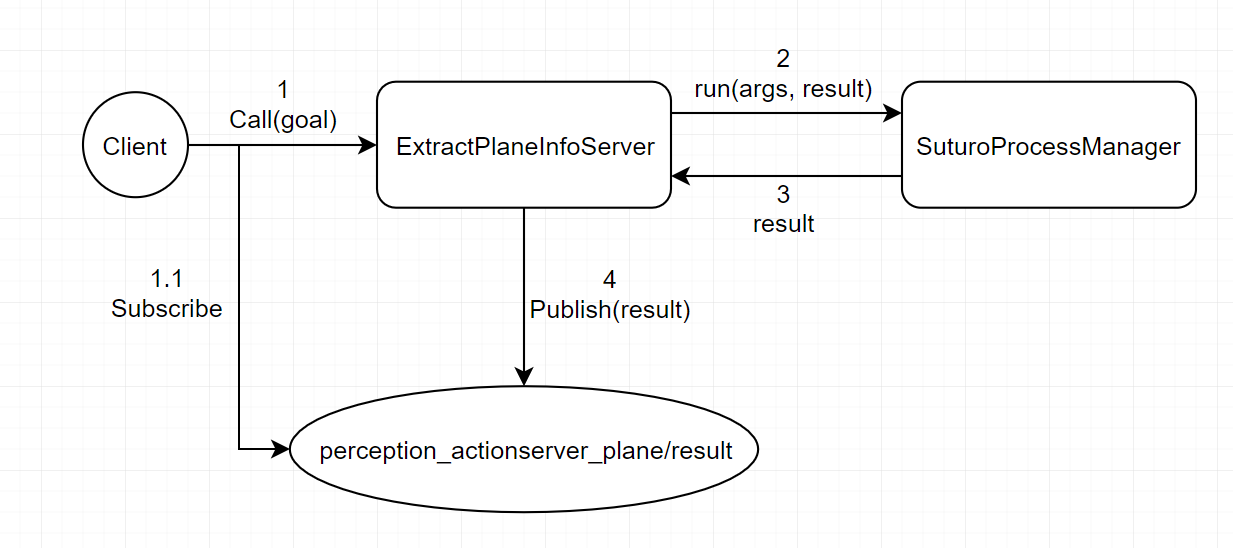
\includegraphics[width=1\textwidth]{pictures/perception/suturo_ExtractPlaneInfoServer.png}
   			 \caption{ExtractPlaneInfoServer}
  			\end{figure}

			\subsection{perception\_server}
perception\_server is the only way to launch \texttt{ExtractObjectInfoServer} and \texttt{ExtractPlaneInfoServer} they cannot be used separated. \\
It works by calling : \texttt{roslaunch rs\_perception hsrb\_perception.launch} in the rs\_perception directory.

		\section{rs\_turn\_table}
		\chapterauthor{Leonidas Paniago}
The package \href{https://github.com/Vanessa-rin/rs_turn_table}{rs\_turn\_table} belongs to the last SUTURO group. There were no big changes to the core code, only small situational changes not implemented on the master. 
This package is mainly for image recording, all recorded images will then be used for object recognition.  
rs\_turn\_table heavily depends on \textit{Openni2} as a driver for the Kinect camera. HSR could be used for the image recording but in reality, it turns out to be really impractical. 
The Kinect camera offers more flexibility and gives other groups more time with the robot. \textit{Openni2} installation was a major problem in the project due to a lack of documentation. For this purpose, there is a 
\href{https://github.com/SUTURO/suturo_perception/blob/Openni2/Openni2/Openni2_Install}{script} that will install all necessary dependencies and automatically enable depth\_registration in the \textit{Openni2} launch file. The camera can be started by calling: \texttt{roslaunch openni2\_launch openni2.launch}
 \\ Note: \textit{Openni2} did not work on a Virtual machine with Ubuntu-16.04.6. The camera goes on but no output is sent to the camera topic. 

			\subsection{Pipeline: estimate\_plane}
This pipeline will save all visible planes, they are callable again. The best way to get a clean plane is to set the Limits on \texttt{PointCloudFilter} by hand. Only one plane should be visible. To start the pipeline run : \texttt{rosrun robosherlock run \_ae:=estimate\_plane \_vis:=true} 
\begin{itemize}
	\item CollectionReader : Takes care of the camera input
	\item ImagePreprocessor : Prepares image for further processing and implement image filters  
	\item PointCloudFilter : Filters points out of the cloud that are not in the range of the given parameters for X, Y and Z axes
	\item PlaneAnnotator : Finds a plane and saves it to a file 
\end{itemize}


			\subsection{Pipeline: save\_images}
This pipeline uses the saved plane from estimate\_plane as base for the image processing and takes periodic images from objects on the plane, if there is more than one cluster visible the annotator will not trigger the saving process. To start the pipeline run : \texttt{rosrun robosherlock run \_ae:=save\_images \_vis:=true} 
\begin{itemize}
	\item CollectionReader : Takes care of the camera input
	\item ImagePreprocessor : Prepares image for further processing and implement image filters  
	\item PointCloudFilter : Filters points out of the cloud that are not in the range of the given parameters for X, Y and Z axes
	\item NormalEstimator : Estimate surface normal's in a PointCloud 
	\item PlaneAnnotator : Finds a plane in the current scene and saves it into the CAS
	\item PointCloudClusterExtractor : Extracts all points found in the PointCloud that are perpendicular to the plane 
	\item SaveClusterCloudsAndImages : Save Information about the Cluster to a file 
\end{itemize}
		\begin{figure}[H]
   			 \centering
    			 \subfigure[Original]{%
            		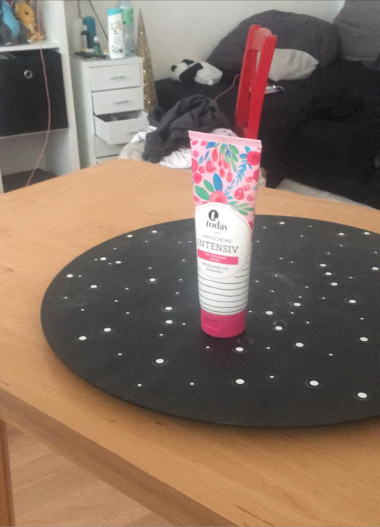
\includegraphics[width=0.5\textwidth]{pictures/perception/turn_table_2.png}
        			}%
        			\subfigure[Pointcloud representation]{%
           		 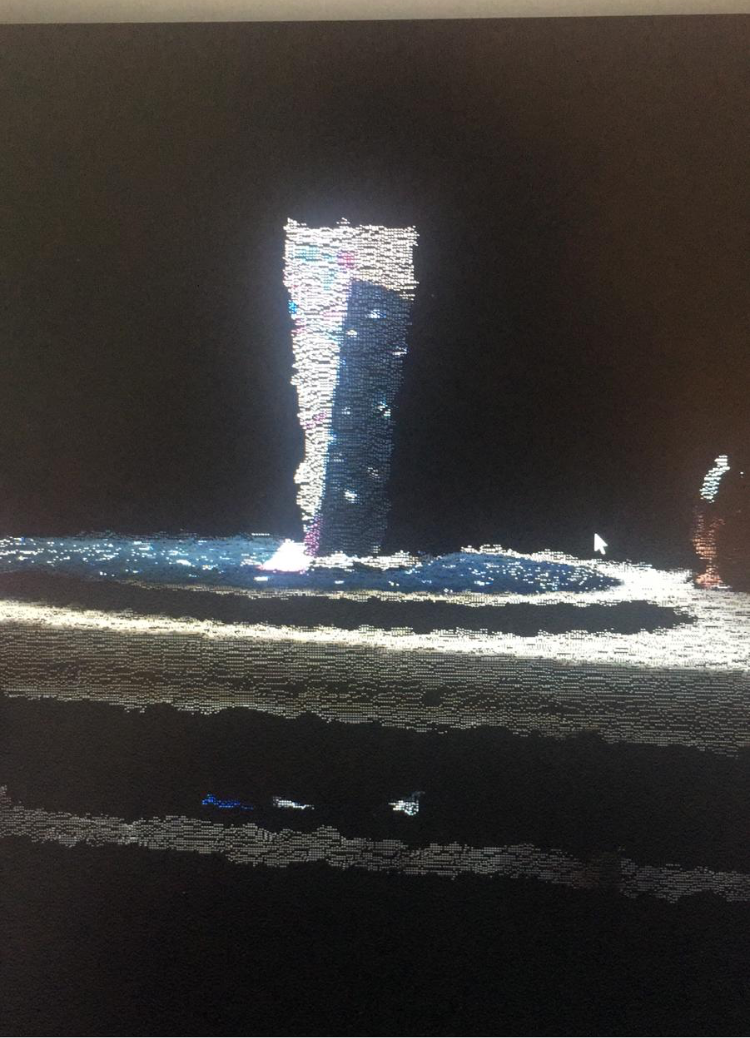
\includegraphics[width=0.5\textwidth]{pictures/perception/turn_table_1.png}
        			}
   			 \caption{Turn table setup}
			  \label{turnTableOriginal}
  		\end{figure}
In picture \ref{turnTableOriginal} the RGB texture and the pointcloud representation do not match fully. This occurs if the unregistered image topic is used for the pipeline. 
		\begin{figure}[H]
   			 \centering
    			 \subfigure[RGB]{%
            		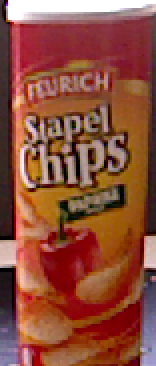
\includegraphics[width=0.5\textwidth]{pictures/perception/Feurich_Stapel_Chips_Paprika_0_4_crop.png}
        			}%
        			\subfigure[Pointcloud representation]{%
           		 
\includegraphics[width=0.5\textwidth]{pictures/perception/Feurich_Stapel_Chips_Paprika_0_3_mask.png}
        			}
   			 \caption{save\_image output}
			 \label{FeurichChips}
  		\end{figure}
The picture \ref{FeurichChips} shows a standard output for the save\_images pipeline.

\section{classificationEvaluation Package}
\chapterauthor{Jan-Frederik Stock}

\subsection{Introduction}
The classificationEvaluation package is used to save and display the classification results of the perception pipeline. The results can be saved in a markdown table and/or be displayed as a scatter plot. It consists mainly of the rsClassificationEvaluator.py python script. Here, the class ResultActionClient is implemented, which serves as an action client for the perception object info action server.\\

\subsection{Motivation}
The classificationEvaluation package was created to access and save the classification results, which was not easily possible at the time. It was also meant as a way to compare classification performance based on the confidence measurements of different algorithms. It became evident in the process that this was not useful, the reason for this will be outlined in the following.\\

After implementing the classificationEvaluation package, it was used to create the plot \ref{fig:k comparison plot}. This plot was meant to compare the performance of a k-nearest-neighbor classifier, with different selections of the parameter k. The value of the k is shown on the x-axis, the confidence is on the y-axis, with zero being the lowest and one being the highest possible confidence. Each point in the plot represents a sample, that was classified.\\

\begin{figure}
	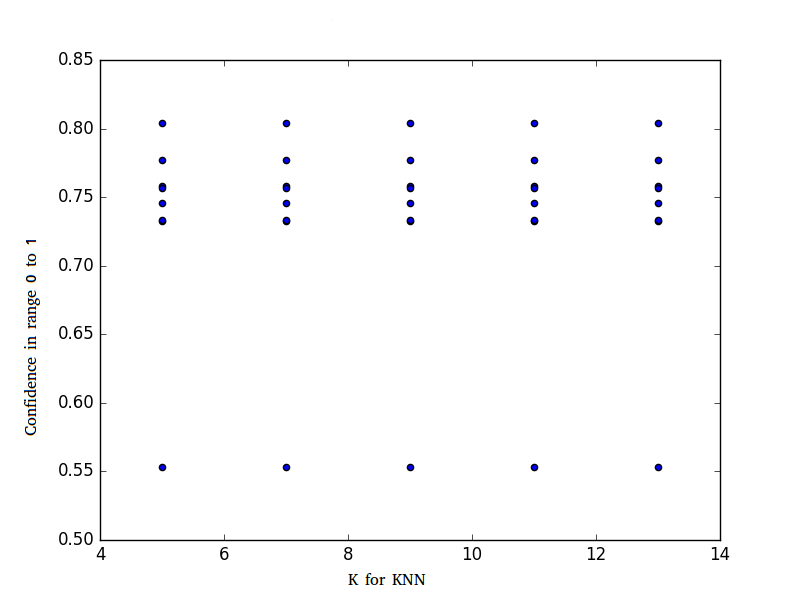
\includegraphics[width=\textwidth]{pictures/perception/k_comparison.png}
	\caption{Plot showing the confidence for different values of k}
	\label{fig:k comparison plot}
\end{figure}

The plot shows that the confidence does not change with different values of k, which is surprising due to the details of the KNN algorithm. The reason for this is the way the confidence was implemented in the KNN classifier:

\begin{lstlisting}
cv::Mat results, neighborResponses, dists;
double res = knncalld->findNearest(test_mat, k_max, results, neighborResponses, dists);
double confidence = (2 - dists.at<float>(0))/2);
\end{lstlisting}

This implementation of the KNN algorithm returns a one dimensional matrix with the distances of each of the k neighbors to the sample. Yet the calculation of the confidence only takes the distance of the first neighbor into consideration. This is why the confidence does not change with the altering of the k. The calculation of the confidence was later changed for the SUTURO project, more details can be found in \ref{KNN confidence}.\\

Regarding the results, evaluating KNN classification performance based on the confidence is very dependent on the implementation of the confidence. The confidence does not necessarily provide a good measurement of the real performance of the algorithm. Comparing based on a confidence might be acceptable for evaluating the best parameters for a specific algorithm, but it is not at all useful to compare different classification algorithms.\\

This is due to the fact that the common classification algorithms work very differently, which makes the implementation of a confidence unique for each algorithm. Because of that, algorithms are not comparable based on confidence. A better and more objective way to compare them was implemented in the SUTURO project and it is described in section \ref{clusterLabeling}.


 

\subsection{The ResultActionClient class}
The class provides the following methods:

\begin{itemize}
\item 
sendGoal(self)\\
This method is used to send a goal to the ExtractObjectInfoServer and thus triggering the pipeline.

\item saveResult(self, result)\\
This method saves the action result, which is the classification, in a field of the class.

\item saveToMd(self, algorithm)\\
This method saves the collected results of the classification in a \textit{markdown} table. If a \textit{markdown} file with the name "\texttt{evaluation.md}" is found in the directory the script is executed in, the results are appended to it, otherwise, the file is created.

\item plotResult(self)\\
The method plots the collected results using the scatter plot function from \texttt{matplotlib}.
\end{itemize}

\subsection{Main method}
The main method tries to create an instance of the \texttt{resultActionClient} class, does some i/o with the user, sets the parameters for the \texttt{resultActionClass}, and then triggers the action. It also uses the provided methods to save the results to a markdown file and plot them.

\section{Feature Extraction Tools}
 \chapterauthor{Jan-Frederik Stock}
Perception uses feature extraction to get quantifiable data from the perceived images. On this data, the classification algorithms can then be trained. Every time a new image is perceived, its features are extracted, which are then used to classify it. Perception uses a neural network without the output layer to extract features, the output of this network are the features. The neural networking framework used for this is \textit{Caffe}, the trained network is the \textit{BVLC Reference Net}. If you want to install \textit{Caffe}, you can find instructions in the SUTURO projects installation guide, in sections 3.2 and 3.3. The tools directory in the \texttt{featureExtraction} package contains the two bash scripts make\_split\_from\_directory.sh and make\_split\_list\_from\_directory.sh.

\subsection{make\_split\_from\_directory.sh} \label{make_split_from_directory}
This bash script can be used to create a split \textit{YAML}-file which is required to perform feature extraction with the rs\_addons package. To use it, the user has to place the file in the parent directory of the directory, in which the folders with the recorded images are stored. When being executed, the script asks for a filename and the name of the directory out of which the \textit{YAML}-file will be created. It then creates the \textit{YAML}-file using the names of the directories in which the images are stored as class names.

\subsection{make\_list\_from\_directory.sh}
This bash script does nearly the same thing as the make\_split\_from\_directory.sh \ref{make_split_from_directory}, except that it does not create a split file but a list of the class names. This is required by the classifying annotator and has to be pasted into the annotators \textit{YAML}-file. The comma after the last class name in the list has to be removed manually.

\section{Classification - Splits}
\chapterauthor{Jan-Frederik Stock}
In order to be able to classify images with rs\_addons and \textit{Caffe}, a split file has to be created, in which the output classes have to be listed. This is essential for the classifier to work. In the beginning of the SUTURO project, the question came up if every recorded object should be represented as its own class for the classfication, or if similiar objects should be consolidated into superclasses, for example into fruits or dishes.\\

The perception group decided to represent every recorded object in its own class. This has numerous advantages:\\

Firsly, the classfication works better done this way, because the classes are more distinct. A superclass holding fruits would contain many differently looking objects, like bananas and apples. These fruits have different colors and shapes, which would mean that the probability of similiar looking items which are not fruits being also labeled as fruit would be higher.

Secondly, more information is available for other processing steps after the perception group. For example, if an object is labeled as a snack, the knowledge group has much less information than if it was labeled as a Pringles can. Representing the Pringles as its own class gives the knowledge group the opportunity to group objects based on their own criteria, for example shape, color, or even the amount of calories a certain type food contains. This would not be possible if objects are just labeled as superclasses.
 



\section{calculateConfidence in RSKNN.cpp}\label{KNN confidence}
\chapterauthor{Jan-Frederik Stock}
In the \texttt{RSKNN.cpp}, implementing KNN-classification in the rs\_addons package, the following method was added:

\begin{lstlisting}
double RSKNN::calculateConfidence(double classificationResult, cv::Mat neighborResponses)
\end{lstlisting}

It calculates the classification confidence for the KNN-classification by dividing the number of neighbors belonging to the result class, by the total number of visited neighbors. 

\section{The clusterLabeling Package}\label{clusterLabeling}
\chapterauthor{Jan-Frederik Stock}
\subsection{Motivation}
The \texttt{clusterLabeling} package fixes a fundamental problem: Before its existence, it was not possible to compare the performance of classifiers objectively. A user could only look at a given classification and decide if the algorithm was working good or bad overall, but not decide on quantitative measurement. The ability to do this is not just important to evaluate the performance of a single algorithm, but even more to compare the performance of different algorithms and select the best one for a specific use case.\\

A very common procedure to do this in machine learning is the evaluation of an algorithm by splitting the available data into a test set and a training set. The available data contains a class label for every sample. The algorithm is trained on the training set and the test set is held back to test the performance. This is done by introducing samples from the test set into the algorithm and then checking if the algorithm produces the correct label. By dividing the number of correctly classified samples by the total number of tested samples, the accuracy is calculated. This is a very common measure of classification performance and it is suitable for a multi class problem like the perception groups task.\\

In the particular case of the SUTURO project, it was not practical to split a test set from our training data, because we recorded the objects by taking pictures in a circle around it. Taking some of these pictures away for testing would mean testing the classification on perspectives that are not represented in the training data, leading to worse classification performance. Also, in the real life application on the robot, the classification has to work on different scenes than the setting of the recording, so it makes sense to test the classification on similar, more realistic scenes. The ability to do this is implemented in the \texttt{clusterLabeling} package. The user is able to test their classification algorithm on scenes recorded on the actual robot they are working with.  

\subsection{Usage}

\subsubsection{The clusterLabeler}
The \texttt{clusterLabeler} is the Annotator used for labeling. It is best placed at the end of your labeling pipeline, which also has to contain the annotators necessary for clustering. The labeling and the evaluation work best if a good clustering is achieved, so it is recommended to use the \texttt{PointCloudFilter} or other filters you may have to ensure this. You must not change the settings of any annotator in the pipeline while creating the labels and using them for the evaluation later, otherwise, it can not be guaranteed that the cluster numbering will stay the same. To be able to label a scene frame by frame, put the Trigger at the beginning of your pipeline. You can use the \texttt{classificationEval} pipeline in the \texttt{rs\_perception} package (\ref{rs_perception}) to start.\\

To label a scene, you start your labeling pipeline and call the trigger service once. You can then chose the \texttt{clusterLabeler} in the visualizer, which will display a number for every cluster. You can see an example of how this looks in figure \ref{fig:clusterLabeler visualization}.
\begin{figure}
  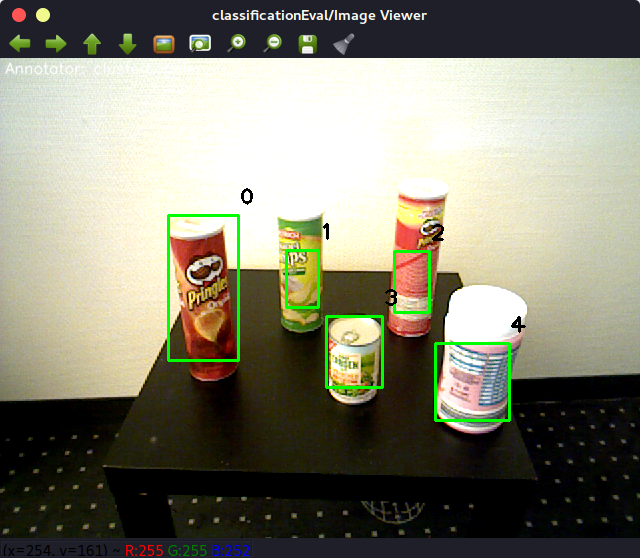
\includegraphics[width=\linewidth]{pictures/perception/cluster_numbering.png}
  \caption{The visual output of the clusterLabeler.}
  \label{fig:clusterLabeler visualization}
\end{figure}

\newpage

Now, you can note the class for every cluster in a labeling \textit{JSON}-file, which has to look like figure \ref{fig:labeling file}. You can also have look at the file already present in the labeling directory in the \texttt{custerLabeling} package for the correct syntax. Now call the trigger service again and proceed to label. If you do not want to create labels for a frame, for example if the clustering is bad, you can just leave the clusters array in the \textit{JSON}-file empty. The \texttt{classificationEvaluationAnnotator} will leave this frame out of the calculation. Currently, one has to create the labeling \textit{JSON}-file by hand, but there is a started implementation for a GUI for this task in the \texttt{clusterLabeling} package.

\begin{figure}
  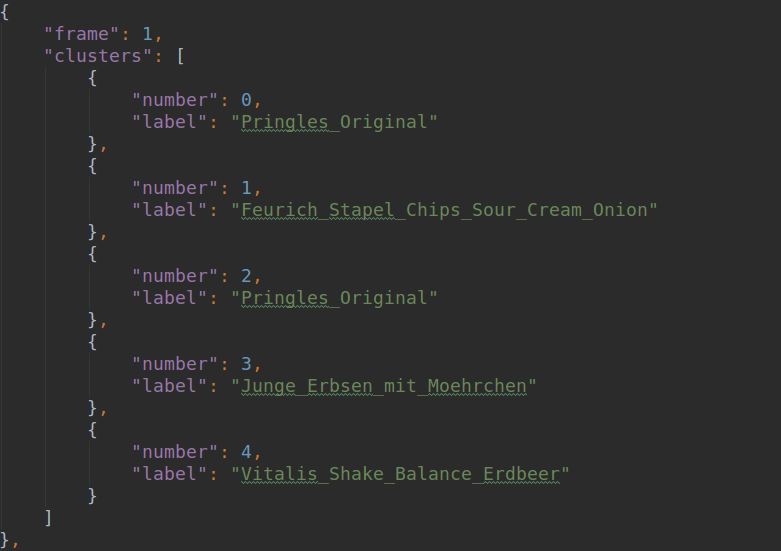
\includegraphics[width=\linewidth]{pictures/perception/labeling_file.png}
  \caption{The \textit{JSON}-file containing the labels.}
  \label{fig:labeling file}
\end{figure}


\subsubsection{classificationEvaluationAnnotator}
The \texttt{classifcationEvaluationAnnotator} can read a labeling file and will then compare the labels with the actual classification to calculate the accuracy. Swap the \texttt{classificationEvaluationAnnotator} with the \texttt{clusterLabelingAnnotator} and add you classifying annotators before it. Do not change anything else about the pipeline. Set the path to your labeling file in the descriptor \textit{YAML}-file of the \texttt{classificationEvaluationAnnotator} and start your pipeline. Trigger the pipeline as many times as you have labeled frames in your \textit{JSON}-File. The \texttt{classificationEvaluationAnnotator} will display the current accuracy in your step in \textit{RoboSherlocks} terminal output. This is shown in figure \ref{fig:classificationEvaluationAnnotator output}.

\begin{figure}
  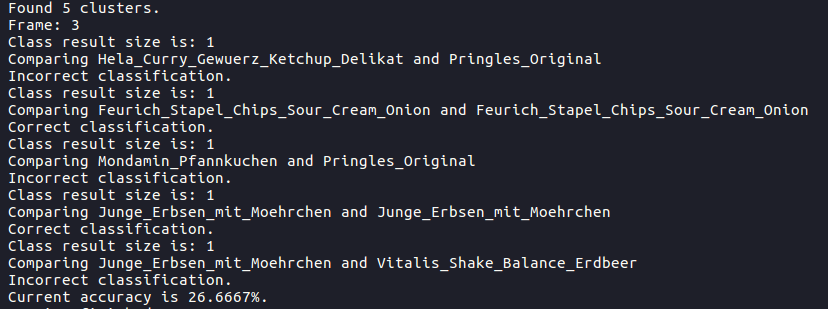
\includegraphics[width=\linewidth]{pictures/perception/accuracy.png}
  \caption{The output of the classificationEvaluationAnnotator.}
  \label{fig:classificationEvaluationAnnotator output}
\end{figure}

\subsection{Documentation}
\subsubsection{clusterLabeler}
\begin{lstlisting}
TyErrorId processWithLock(CAS \&tcas, ResultSpecification const \&res_spec)
\end{lstlisting}
This is the main processing method of the annotator.\\

Firstly, it gets the detected clusters from \textit{RoboSherlocks} central data structure like this: \label{getting the detected clusters.}

\begin{lstlisting}
//Get the clusters in the image found by previous annotators
std::vector<rs::ObjectHypothesis> clusters;
scene.identifiables.filter(clusters);
\end{lstlisting}

It then iterates over the found clusters and draws a rectangle around every found cluster with a number next to it, corresponding to its position in the clusters vector. If the filtering settings are not changed for the pipeline, this order does not change.

\begin{lstlisting}
//set region of interest for the cluster
rs::ImageROI cluster_roi = cluster->rois.get();
//create Rectangle
cv::Rect rectangle;
rs::conversion::from(cluster_roi.roi.get(), rectangle);
//Draw the numbering for the cluster
drawCluster(current_image, rectangle, std::to_string((cluster - clusters.begin())));
\end{lstlisting}

\begin{lstlisting}
static void drawCluster(cv::Mat input, cv::Rect rectangle, const std::string &label)
\end{lstlisting}

This is a helper function that creates the rectangle for the picture and inserts it into the matrix holding the picture of the scene, as well as the number:

\begin{lstlisting}
cv::putText(input, text, cv::Point(rectangle.x + rectangle.width, rectangle.y - offset - textSize.height), cv::FONT_HERSHEY_PLAIN, 1.5, CV_RGB(0, 0, 0), 2.0);
\end{lstlisting}

This will then be displayed in \textit{RoboSherlocks} viewer.



\subsubsection{classificationEvaluationAnnotator}
The annotator class contains fields holding the path to the labeling file, a rapid\textit{JSON} document, which will later contain the object representation of the parsed \textit{JSON}-file and fields used to calculate the accuracy.

\begin{lstlisting}
TyErrorId initialize(AnnotatorContext \&ctx)
\end{lstlisting}

This method is executed at the startup of the pipeline.  It gets the path to the labeling file from the \textit{YAML} description and reads the file. The file is then parsed into a \textit{JSON} object representation by rapid\textit{JSON} and saved in a field of the class, like so:

\begin{lstlisting}
document.Parse(content.c_str());
\end{lstlisting}

\begin{lstlisting}
TyErrorId process(CAS \&tcas, ResultSpecification const \&res_spec)
\end{lstlisting}

This is the main processing method of the annotator. It gets the identified clusters from the central \textit{RoboSherlock} data structure like the clusterLabeler \ref{getting the detected clusters.}. It then checks, if the \textit{JSON}-file has an entry for the current frame: 

\begin{lstlisting}
if (!document["clusterLabeling"][framecounter]["clusters"].Empty())
\end{lstlisting}

This allows for frames that have bad clustering to be skipped for the evaluation, as a good clustering is a prerequisite for the classification. If the \textit{JSON}-file contains a labeling for the current frame, the method loops through the found clusters. In the loop, it first gets the classification from the algorithm under evaluation from RoboSherlocks central data strucutre:

\begin{lstlisting}
std::vector<rs::Classification> classResult;
clusters[i].annotations.filter(classResult);
\end{lstlisting}

If this result is not empty, the method compares it to the label from the \textit{JSON}-file:

\begin{lstlisting}
if (classResult[0].classname.get().compare(
                          document["clusterLabeling"][framecounter]["clusters"][i]["label"].GetString()) == 0)
\end{lstlisting}

The classification result can be empty if the classification algorithm filters out results not passing a certain confidence threshold. This is counted as an incorrect classification.\\

If the classes match, the number of correctly classified samples is incremented, as well as the total number of samples. If not, just the total number of samples is incremented.\\

After the loop, the accuracy at the current point of the calculation is calculated by dividing the number of correctly classified samples by the total number of samples:

\begin{lstlisting}
accuracy = ((float) correct_samples) / ((float) total_samples);
\end{lstlisting}

In the end, the frame counter is incremented and the calculation starts again for the next frame.

\section{SuturoShapeAnnotator}
\chapterauthor{Evan Kapitzke}

\subsection{Motivation}
The implementation of an additional annotator to classify basic shapes was motivated by the fact that a huge amount of our processing time
was used by the \textit{PrimitiveShapeAnnotator}. Object shapes are used to determine which type of basic model is used to spawn it in the Planning and Knowledge world representation.

\subsection{Implementation}
The \textit{SuturoShapeAnnotator} uses three different types of SAC models to determine the shape of an object.
The point clouds are processed parallel in order to minimize the amount of time that is needed to process all clouds in our current scene.
For each object the functions \textit{annotateBox(..), annotateCylinder(..)} and \textit{annotateSphere(..)} are called and the result with the highest confidence
will be selected as result. \textit{annotateBox(..)} tries to find a plane that is orientated in an particular angle to the camera. 
The other two functions fit their corresponding SAC model.

\begin{itemize}
\item drawResult(rect, result\_name, confidence, color)\\
Draws the result for a cluster in the given rectangle.

\item annotateBox(tcas, clusterCloud, clusterNormals)\\
Segments planes that are in a given angle to the camera. The confidence describes how many inliers are found. Returns the confidence as a result.

\item annotateCylinder(tcas, clusterCloud, clusterNormals)\\
Segments cylinder models. The confidence describes how many inliers are found. Returns the confidence as a result.

\item annotateSphere(tcas, clusterCloud, clusterNormals)\\
Segments sphere models. The confidence describes how many inliers are found. Returns the confidence as a result.

\item initialize(ctx)\\
Initializes the drawing annotator.

\item processWithLock(tcas, res\_spec)\\
Iterates over all clusters and executes the segmentation on them. The result with the highest confidence will be annotated if
the confidence is over the minimum threshold. The threshold can be set in the according \textit{YAML} descriptor.
\end{itemize}

\subsection{Performance}
The main goal was to increase performance. The comparison of the annotators focuses on execution time.
Three scenes are used to evaluate the results of both annotators and their execution time.

\subsubsection{Scene: Shelve}
The first scene consists of multiple objects which are placed in a shelve.
\begin{figure}
  \center
  \includegraphics[width=0.5\textwidth]{pictures/perception/shape_annotator/classification_test_shelve/primitive.png}
  \caption{PrimitiveShapeAnnotator}
  \label{fig:shapeAnnotatorShelvePrimitive}
\end{figure}
\begin{figure}
  \center
  \includegraphics[width=0.5\textwidth]{pictures/perception/shape_annotator/classification_test_shelve/suturo.png}
  \caption{SuturoShapeAnnotator}
  \label{fig:shapeAnnotatorShelveSuturo}
\end{figure}

The following graph shows how long it takes to process one frame for each annotator.
{\center
  \includegraphics[width=1.2\textwidth]{pictures/perception/shape_annotator/classification_test_shelve/chart.png}
}
\newpage

\subsubsection{Scene: Table}
In the second scene multiple objects are placed on a table.
\begin{figure}
  \center
  \includegraphics[width=0.5\textwidth]{pictures/perception/shape_annotator/classification_test_table/primitive.png}
  \caption{PrimitiveShapeAnnotator}
  \label{fig:shapeAnnotatorShelvePrimitive}
\end{figure}
\begin{figure}
  \center
  \includegraphics[width=0.5\textwidth]{pictures/perception/shape_annotator/classification_test_table/suturo.png}
  \caption{SuturoShapeAnnotator}
  \label{fig:shapeAnnotatorShelveSuturo}
\end{figure}

The following graph shows how long it takes to process one frame for each annotator.
{\center
  \includegraphics[width=1.2\textwidth]{pictures/perception/shape_annotator/classification_test_table/chart.png}
}
\newpage

\subsubsection{Scene: Training}
Again multiple objects are placed on a table.
\begin{figure}
  \center
  \includegraphics[width=0.5\textwidth]{pictures/perception/shape_annotator/classification_test_training/primitive.png}
  \caption{PrimitiveShapeAnnotator}
  \label{fig:shapeAnnotatorShelvePrimitive}
\end{figure}
\begin{figure}
  \center
  \includegraphics[width=0.5\textwidth]{pictures/perception/shape_annotator/classification_test_training/suturo.png}
  \caption{SuturoShapeAnnotator}
  \label{fig:shapeAnnotatorShelveSuturo}
\end{figure}

The following graph shows how long it takes to process one frame for each annotator.
{\center
  \includegraphics[width=1.2\textwidth]{pictures/perception/shape_annotator/classification_test_training/chart.png}
}

\subsubsection{Conclusion}
The \textit{SuturoShapeAnnotator} processes cluster way faster than the \textit{PrimitiveShapeAnnotator}. In addition, the results are more accurate.
On average the \textit{SuturoShapeAnnotator} is about fifth-teen times faster than the \textit{PrimitiveShapeAnnotator}.

\section{rs\_hsrb\_perception Package}
\chapterauthor{Evan Kapitzke}

The \texttt{rs\_hsrb\_perception} package was created in the Suturo Master-project. The package implements a \textit{RoboSherlock} process manager, called the\\ \texttt{SuturoProcessManager}. Additionally, it contains modified annotators to annotate regions.

\subsection{RegionAnnotator}
\begin{itemize}
\item TyErrorId process(tcas, res\_spec)\\
Iterates through the clusters that are currently saved in the CAS and annotates the region in which they are presently based on the cluster pose.
This method only got changed to work with the \textit{RoboSherlock} master.
\end{itemize}

\subsection{SuturoProcessManager}
In order to reconfigure annotators and to properly convert the information where it was generated a new process manager was necessary.
The \textit{SuturoProcessManager} already existed because the last SUTURO group created it to detect whether or not a shelf door is open.
The process manager organizes the results of the perception pipeline and returns them as \textit{ObjectDetectionData} messages.
The standard \textit{RSProcessManager} is unable to create custom messages.

\begin{itemize}
\item setup()\\
Creates the ressource manager and instantiates the region vector.

\item init(pipeline)\\
Initializes the given pipeline (aggregate analysis engine \textit{YAML} descriptor) and starts the visualizer.
This method got changed to allow the visualization of the pipeline.

\item run(args, detectionData)\\
Executes the initialized pipeline once with the given arguments and saves the result in detectionData.
This method now checks for the region "robocup\_default" and disables the region filter to perceive objects that can not be found
in a region. For example, a Pringles can that is placed on the ground.

\item has\_vertical\_plane()\\
Returns true if the current CAS contains a vertical plane.

\item getClusterFeatures(cluster, data)\\
Extracts the annotations of the given cluster and generates an ObjectDetectionData object. 
This object will be added to the data pointer. makeObjectDetectionData(...) from suturo\_conversion is used.
Currently, only one KnnAnnotator (for known objects) is used to determine the class label of an object.

\item visControlCallback(req, res)\\
Callback for navigation through the different annotation previews in the visualization window.
\end{itemize}

\subsection{SuturoRegionFilter}
\subsubsection{Prerequisites}
The robot must be orientated correctly and the correct semantic map needs to be set.
The names of the default regions must be the same as in the semantic map definition.
RVIZ is able to update the robot orientation by executing a 2D-Pose-Estimate. The robot must be orientated manually.

The \texttt{SuturoRegionFilter} uses the information from \texttt{suturo\_semantic\_map.yaml} to create the regions. 
The \texttt{suturo\_semantic\_map.\textit{YAML}} is created by the \texttt{region\_filter\_setup.py}. 
This script translates all information about regions position and orientation from knowledge in to a usable \textit{YAML} file. 
This is necessary because this data is defined differently for each group.

\subsubsection{Implementation}
Adapted region filter from RoboSherlock. In order to perceive objects on the ground, it is necessary to disable
the region filtering as long as no ground region is defined. To allow the perception of objects on every surface
without restarting the perception pipeline, the method \texttt{reconfigure()} got implemented in our own copy of the 
\texttt{RegionFilter}. The reconfiguration function updates all parameters based on the current annotator context.
To enable or disable the region filter the \texttt{SuturoProcessManager} overwrites an parameter in the \texttt{SuturoRegionFilter}
and calls \texttt{reconfigure()} on it. 
This allows the process manager to temporarily disable the functionality of the annotator without restarting the pipeline if the need arises.

\begin{itemize}
\item reconfigure()\\
Reconfigures the annotator to disable/enable its functionality without restarting the pipeline or removing it.
\end{itemize}

\subsection{suturo\_conversion}
Implements template functions to convert from and to PoseStamped objects.
Following functions got changed:

\begin{itemize}
\item decode\_shape(shapes)\\
Converts the result of the \texttt{PrimitiveShapeAnnotator} to match the required shape format in the \texttt{ObjectDetectionData} object.

\item makeObjectDetectionData(pose, geometry, shape, objClass, confidence, c, odd)\\
Combines the given parameters to an \texttt{ObjectDetectionData} message.
\end{itemize}

\subsubsection{ObjectDetectionData}
The \textit{ObjectDetectionData} message will be used to send the results of the perception pipeline to Planning and Knowledge.

\begin{lstlisting}
# Communicated via actionserver at topic /perception_actionserver/result
string name
string obj_class
float64 confidence_class

uint8 shape # and the shape (please, if possible, as fallback if confidence is low). 
float64 confidence_shape

geometry_msgs/PoseStamped pose
float64 width
float64 height
float64 depth

std_msgs/ColorRGBA color
float64 confidence_color

string region

# Shape values
uint8 ARROW=0 # Not used
uint8 CUBE=1
uint8 SPHERE=2
uint8 CYLINDER=3
\end{lstlisting}

			\section{rs\_Athene}
			\chapterauthor{Leonidas Paniago De Oliveira Neto}
There is a sub-branch of our GitHub named \href{https://github.com/SUTURO/suturo_perception/tree/Handcamera_tracking}{Handcamera\_tracking}
which includes \texttt{rs\_Athene} and all following featured annotators. 
None of them made it to the main branch because they were not finished or were not suitable for any current task. \\
Each annotator can be executed by enabling the corresponding annotator in the descriptor \texttt{athene.yaml} and running : \texttt{rosrun robosherlock run \_ae:=athene}. 

				\subsection{TwoDAnnotator}
The \href{https://github.com/SUTURO/suturo_perception/blob/Handcamera_tracking/rs_Athene/src/TwoDAnnotator.cpp}{TwoDAnnotator} is responsible for shape recognition that should replace the old \texttt{ShapeAnnotator} by improving the accuracy, reducing processing time, and expanding the usability. 
There are two main concerns with the old annotator. First, the annotator needs a long time to process the data and the results are not ideal. Second, the annotator only process RGB-D images (color and dense depth images). The only camera capable of RGB-D images is the Head-camera, all other cameras can not be used. \\
To fix these issues, the \texttt{TwoDAnnotator} uses only RGB (color images) images, which makes the processing less demanding than there's fewer data to process. Furthermore, all the HSR cameras are usable for shape recognition because each one is capable of outputting RGB images. \\
The TwoDAnnotator works by converting the RGB image to grayscale :
\begin{lstlisting}
..
cas.get(VIEW_COLOR_IMAGE, src); 
..
cv.cvtColor(src, src_gray, CV_BGR2GRAY);
..
\end{lstlisting}
Then smoothing the grayscale output for better results : 
\begin{lstlisting}
..
//thresholding the grayscale image to get better results
cv.threshold(src_gray, src_gray, thresh, maxval, type);
..
//smooth the original image using Gaussian kernel to remove noise
cv.GaussianBlur(src_gray, src_gray, Size(9, 9), 0);
..
\end{lstlisting}
The output is used for edge detection by running the canny-algorithm : 
\begin{lstlisting}
..
cv.Canny(src_gray, canny_output, thresh, thresh * 2, 3);
..
\end{lstlisting}
All found edges are then used for the contour analysis : 
\begin{lstlisting}
..
cv.findContours(canny_output, contours, hierarchy, CV_RETR_TREE, CV_CHAIN_APPROX_SIMPLE, Point(0, 0));
..
\end{lstlisting}
Each contour gets checked for the number of edges. For three edges it is assumed as triangle, four edges implies a square. In addition, each contour needs to reach a certain area threshold. The triangle areas get checked using the Hero's formula, squares using Bretschneider formula. \\
\begin{lstlisting}
..
double area = sqrt((a + b + c)*(a + b - c)*(b + c - a)*( c+ a - b))/4;
..
double area = sqrt((4*pow(e,2)*pow(f,2)) - pow((pow(b,2) + pow(d,2) - pow(a,2) - pow(c,2)),2))/4;
..
\end{lstlisting}

Circles are are treated separately using Hough Circle Transform on the grayscale image : 

\begin{lstlisting}
..
cv.HoughCircles( src_gray, circles, CV_HOUGH_GRADIENT, 1, src_gray.rows/8, 200, 100, 0, 0 );
..
\end{lstlisting}

The \texttt{TwoDAnnotator} utilizes many functions from the \textit{OpenCV} library, they can be recognized by the cv. prefix. \\ \\
During functionality testing, it turns out that the Hough Circle Transform used to find circles is in the current form to slow. The whole annotator is way too unstable to be used in a real environment. It did not bring any improvement over the old \texttt{ShapeAnnotator} and need further work to be usable. Some form of edge smoothing and a better way to classify triangles and squares could bring better result but in the end, this approach was no longer needed and was discarded.
\begin{figure}[H]
\centering
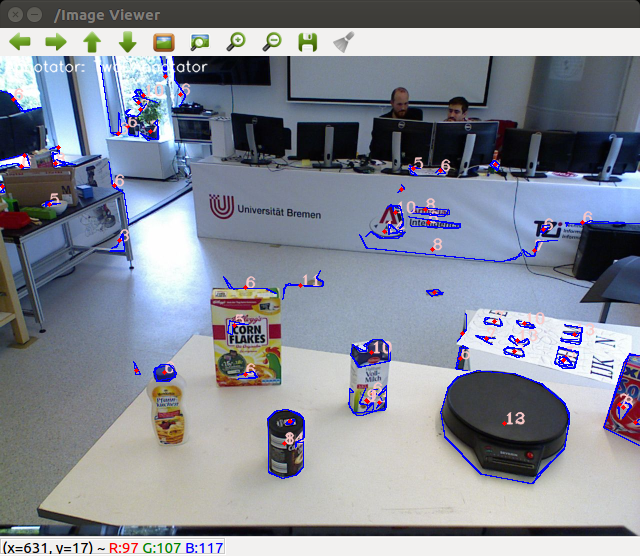
\includegraphics[width=1\textwidth]{pictures/perception/TwoDAnnotator.png}
\caption{TwoDAnnotator output example}
\end{figure}
				\subsection{YOLO}
The \href{https://github.com/SUTURO/suturo_perception/blob/Handcamera_tracking/rs_Athene/src/Yolo.cpp}{YOLO} annotator is as the name suggests, an implementation for the You Only Look Once network. It contains all the needed code for the network to work.
But due to ROS not supporting \textit{OpenCV} latest version, there is no way to execute the annotator. It can be said that the algorithm will work if the supported version of ROS gets updated. Then a similar approach was utilized in the \textit{GoogLeNet} annotator which succeeded and the created YOLO prototype worked like intended.
The approach is based on a python example and works by loading a pre-trained network : 
\begin{lstlisting}
..
// Load names of classes
ifstream ifs(classesFile.c_str());
string line;
while (getline(ifs, line)) classes.push_back(line);
..
// Load the network
Net net = readNetFromDarknet(modelConfiguration, modelWeights);
net.setPreferableBackend(DNN_BACKEND_DEFAULT);
net.setPreferableTarget(DNN_TARGET_CPU);
..
\end{lstlisting}
And feeding it with RGB images : 
\begin{lstlisting}
..
// get frame from the video
cas.get(VIEW_COLOR_IMAGE, frame);
..
// Create a 4D blob from a frame.
blob = blobFromImage(frame, 1/255.0, cvSize(inpWidth, inpHeight), Scalar(0,0,0), true, false);
        
//Sets the input to the network
net.setInput(blob);
..
net.forward(outs, getOutputsNames(net));
\end{lstlisting}

The output consists of all found classes and their bounding boxes that are over a set threshold.
In addition to classification, the prototype calculated the distance from each bounding box center to the image center. 
Then the main focus for this annotator was, getting feedback on the current object position in relation to the camera center.

\begin{figure}[H]
\centering
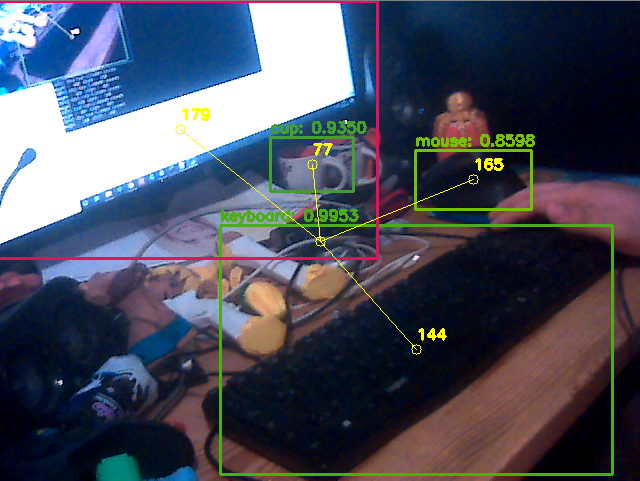
\includegraphics[width=1\textwidth]{pictures/perception/YOLO.png}
\caption{\textit{Python} prototype output}
\end{figure}

				\subsection{GoogLeNet}
\href{https://github.com/SUTURO/suturo_perception/blob/Handcamera_tracking/rs_Athene/src/GoogLeNet.cpp}{GoogLeNet} is an annotator with a similar approach to the YOLO annotator. Both networks use RGB images with the advantage that GoogLeNet runs on an older OpenCV version compatible with ROS.
The \textit{RoboSherlock} implementation uses the trained network to classify objects. The whole class structure is very similar to the YOLO annotator then OpenCV uses the same framework for all supported network architectures. \\
First the pretrained network get loaded: 
\begin{lstlisting}
.. 
// Load serialized model from disk
net = readNetFromCaffe(prototxtpath, modelPath);
..
// Load class names 
ifstream ifs(classesFile.c_str());
string line;
while(getline(ifs, line)){
   ..
   classes.push_back(resultS);
}
..
\end{lstlisting}
And then the input image get set : 
\begin{lstlisting}
..
// Get Image 
cas.get(VIEW_COLOR_IMAGE, frame);
..
// Create a 4D blob from a frame.
blob = blobFromImage(frame, 1, cvSize(inpWidth, inpHeight), Scalar(104, 117, 123), true, false);
..
// set the blob as input to the network and perform a forward-pass
net.setInput(blob);
result = net.forward();
..
\end{lstlisting}
GoogLeNet differs from YOLO by only outputting the class probability so there is no information about where the classes are in the image. The lack of information about the object position makes the annotator useless for tracking. It is nevertheless a powerful tool for the classification of objects. 

				\subsection{PythonEmbedding}
\href{https://github.com/SUTURO/suturo_perception/blob/Handcamera_tracking/rs_Athene/src/PythonEmbedding.cpp}{PythonEmbedding} annotator is an example of how a "Python pure embedding" (calling python script during runtime in c++) can be implemented in \textit{RoboSherlock}. The annotator converts the basic image container \texttt{Mat} to NumPy array : 
\begin{lstlisting}
..
//Get image
Mat src;
cas.get(VIEW_COLOR_IMAGE, src);
..
// copy the data from the cv::Mat object into the array
std::memcpy(m, src.data, nElem * sizeof(uchar));

// the dimensions of the matrix
npy_intp mdim[] = { src.rows, src.cols };
    
// convert the cv::Mat to numpy.array
PyObject* mat = PyArray_SimpleNewFromData(2, mdim, NPY_UINT8, (void*) m);
..
\end{lstlisting}

The script “Hello\_World.py” will be loaded :  

\begin{lstlisting}
..
pModule = PyImport_Import(pName);
..
\end{lstlisting}
And the only existing function "start" get called with the created numpy image : 
\begin{lstlisting}
..
//Search for function
pFunc = PyObject_GetAttrString(pModule, "start");
..
//Set variables
pArgs = NULL;
//Call function with Args
pValue = PyObject_CallObject(pFunc, args);
..
\end{lstlisting}
The \textit{Python} script will then open a new window with the send image.\\
The current version of \textit{RoboSherlock} does not support \textit{Python} annotators, \textit{Python} pure embedding could represent an interim solution to this problem.

\endgroup
\end{document}


